\documentclass[a4paper,12pt]{article}
\usepackage{czech}
\usepackage[utf8]{inputenc}
\usepackage{a4wide}
\usepackage[dvipdfm]{graphicx}
\usepackage{graphics}
\usepackage{indentfirst}
\usepackage{fancyhdr}
\usepackage{setspace}
\usepackage{amsmath}
\usepackage{amssymb}
\usepackage{epsfig}

%%\usepackage{nopageno}
%%\usepackage{txfonts}
\usepackage[usenames]{color}
\renewcommand{\d}{\mbox{d}}

\begin{document}
\section{Úkol}
\begin{enumerate}
\item Pomocí ionizační komory (IK) zjistěte, který z přiložených vzorků radioaktivních zářičů má větší aktivitu.
\item Změřte V-A charakteristiky IK v rozsahu 0-500 V při různých vzdálenostech elektrod 1-6 cm. Použijte intenzivnější zářič.
\item Identifikujte charakteristické oblasti V-A závislosti. Určete optimální napětí a optimální vzdálenost IK.
\item Změřte poměr aktivit přiložených zářičů, odhadněte jejich absolutní aktivity (střední energie vytvoření iontového páru ve vzduchu je 35 eV). 
Stanovte dosah $\alpha$-částic.
\item Pomocí osciloskopu změřte závislost amplitudy elektrického impulzu Geiger-Müllerova (GM) detektoru na napětí v rozsahu 0-1500 V. 
Nepřekračujte napětí 1500 V.
\item Identifikujte charakteristickou oblasti V-A závislosti GM detektoru.
\end{enumerate}

\section{Teorie}
Při průchodu $\alpha$-částice vzuchem dochází k jeho ionizaci. Tím $\alpha$-částice ztrácí kinetickou energii dokud nezastaví. Díky tomu vzniká elektrická 
nerovnováha v oblasti, kterou prošla a tím roste vodivost tohoto prostředí. 
Při přivedení elektrického pole tak mlžeme detekovat prostřednictív tekoucího proudu procházející $\alpha$-částice. Nejedonuší použití tohoto jevu je IK. O něco složitější konstrukci potom reprezentuje GM.

\section{Měření}
\subsection{Aktivita zářičů}
Vzdálenost elektrod v IIK jsem nastavil na 6 cm. Následně jsem změřil oba vzodky při napětí 500 V. Naměřené proudy byly
\begin{eqnarray}
I_1=(0.8\pm 0.3) \mbox{fA}
I_2=(10 \pm 5) \mbox{fA}
\end{eqnarray}
což jasně vypovídá o značně vyšší aktivitě druhého vzorku.

\subsection{V-A charakteristika}
Následně jsem s intenzivnějším zářičem proměřil V-A charakteristiku při vzdálenosti elektrod 1 a 6 cm. Výsledky jsou v tabulce \ref{tVA} a výsledná 
závislost je na obrázku \ref{gVA}.

\begin{table}
$$
\begin{array}{|c|c|c|}
\hline
U/\mbox{V}& 6 \mbox{cm}&    1 \mbox{cm} \\ \hline
500&0.0100&0.0052\\ \hline
400&0.0100&0.0052\\ \hline
300&0.0100&0.0054\\ \hline
200&0.0100&0.0052\\ \hline
100&0.0094&0.0051\\ \hline
90&0.0093&0.0049\\ \hline
80&0.0092&0.0049\\ \hline
70&0.0092&0.0050\\ \hline
60&0.0090&0.0054\\ \hline
50&0.0084&0.0052\\ \hline
40&0.0078&0.0050\\ \hline
30&0.0073&0.0048\\ \hline
20&0.0055&0.0045\\ \hline
10&0.0031&0.0039\\ \hline
9&0.0026&0.0038\\ \hline
8&0.0020&0.0037\\ \hline
7&0.0013&0.0036\\ \hline
6&0.0007&0.0034\\ \hline
5&0.0002&0.0030\\ \hline
4&-0.0001&0.0026\\ \hline
3&-0.0010&0.0014\\ \hline
2&-0.0024&-0.0005\\ \hline
1&-0.0055&-0.0021\\ \hline
0&-0.0046&-0.0035\\ \hline
\end{array}
$$
\caption{V-A charakteristika pro silnější vzorek}
\label{tVA}
\end{table}

\begin{figure}
\begin{center}
% GNUPLOT: LaTeX picture with Postscript
\begingroup
  \makeatletter
  \providecommand\color[2][]{%
    \GenericError{(gnuplot) \space\space\space\@spaces}{%
      Package color not loaded in conjunction with
      terminal option `colourtext'%
    }{See the gnuplot documentation for explanation.%
    }{Either use 'blacktext' in gnuplot or load the package
      color.sty in LaTeX.}%
    \renewcommand\color[2][]{}%
  }%
  \providecommand\includegraphics[2][]{%
    \GenericError{(gnuplot) \space\space\space\@spaces}{%
      Package graphicx or graphics not loaded%
    }{See the gnuplot documentation for explanation.%
    }{The gnuplot epslatex terminal needs graphicx.sty or graphics.sty.}%
    \renewcommand\includegraphics[2][]{}%
  }%
  \providecommand\rotatebox[2]{#2}%
  \@ifundefined{ifGPcolor}{%
    \newif\ifGPcolor
    \GPcolorfalse
  }{}%
  \@ifundefined{ifGPblacktext}{%
    \newif\ifGPblacktext
    \GPblacktexttrue
  }{}%
  % define a \g@addto@macro without @ in the name:
  \let\gplgaddtomacro\g@addto@macro
  % define empty templates for all commands taking text:
  \gdef\gplbacktext{}%
  \gdef\gplfronttext{}%
  \makeatother
  \ifGPblacktext
    % no textcolor at all
    \def\colorrgb#1{}%
    \def\colorgray#1{}%
  \else
    % gray or color?
    \ifGPcolor
      \def\colorrgb#1{\color[rgb]{#1}}%
      \def\colorgray#1{\color[gray]{#1}}%
      \expandafter\def\csname LTw\endcsname{\color{white}}%
      \expandafter\def\csname LTb\endcsname{\color{black}}%
      \expandafter\def\csname LTa\endcsname{\color{black}}%
      \expandafter\def\csname LT0\endcsname{\color[rgb]{1,0,0}}%
      \expandafter\def\csname LT1\endcsname{\color[rgb]{0,1,0}}%
      \expandafter\def\csname LT2\endcsname{\color[rgb]{0,0,1}}%
      \expandafter\def\csname LT3\endcsname{\color[rgb]{1,0,1}}%
      \expandafter\def\csname LT4\endcsname{\color[rgb]{0,1,1}}%
      \expandafter\def\csname LT5\endcsname{\color[rgb]{1,1,0}}%
      \expandafter\def\csname LT6\endcsname{\color[rgb]{0,0,0}}%
      \expandafter\def\csname LT7\endcsname{\color[rgb]{1,0.3,0}}%
      \expandafter\def\csname LT8\endcsname{\color[rgb]{0.5,0.5,0.5}}%
    \else
      % gray
      \def\colorrgb#1{\color{black}}%
      \def\colorgray#1{\color[gray]{#1}}%
      \expandafter\def\csname LTw\endcsname{\color{white}}%
      \expandafter\def\csname LTb\endcsname{\color{black}}%
      \expandafter\def\csname LTa\endcsname{\color{black}}%
      \expandafter\def\csname LT0\endcsname{\color{black}}%
      \expandafter\def\csname LT1\endcsname{\color{black}}%
      \expandafter\def\csname LT2\endcsname{\color{black}}%
      \expandafter\def\csname LT3\endcsname{\color{black}}%
      \expandafter\def\csname LT4\endcsname{\color{black}}%
      \expandafter\def\csname LT5\endcsname{\color{black}}%
      \expandafter\def\csname LT6\endcsname{\color{black}}%
      \expandafter\def\csname LT7\endcsname{\color{black}}%
      \expandafter\def\csname LT8\endcsname{\color{black}}%
    \fi
  \fi
  \setlength{\unitlength}{0.0500bp}%
  \begin{picture}(7200.00,5040.00)%
    \gplgaddtomacro\gplbacktext{%
      \csname LTb\endcsname%
      \put(1342,704){\makebox(0,0)[r]{\strut{}-0.008}}%
      \put(1342,1111){\makebox(0,0)[r]{\strut{}-0.006}}%
      \put(1342,1518){\makebox(0,0)[r]{\strut{}-0.004}}%
      \put(1342,1925){\makebox(0,0)[r]{\strut{}-0.002}}%
      \put(1342,2332){\makebox(0,0)[r]{\strut{} 0}}%
      \put(1342,2740){\makebox(0,0)[r]{\strut{} 0.002}}%
      \put(1342,3147){\makebox(0,0)[r]{\strut{} 0.004}}%
      \put(1342,3554){\makebox(0,0)[r]{\strut{} 0.006}}%
      \put(1342,3961){\makebox(0,0)[r]{\strut{} 0.008}}%
      \put(1342,4368){\makebox(0,0)[r]{\strut{} 0.01}}%
      \put(1342,4775){\makebox(0,0)[r]{\strut{} 0.012}}%
      \put(1474,484){\makebox(0,0){\strut{} 1}}%
      \put(3272,484){\makebox(0,0){\strut{} 10}}%
      \put(5071,484){\makebox(0,0){\strut{} 100}}%
      \put(6869,484){\makebox(0,0){\strut{} 1000}}%
      \put(308,2739){\rotatebox{-270}{\makebox(0,0){\strut{}$I$/nA}}}%
      \put(4171,154){\makebox(0,0){\strut{}$U$/V}}%
    }%
    \gplgaddtomacro\gplfronttext{%
      \csname LTb\endcsname%
      \put(2134,4602){\makebox(0,0)[r]{\strut{}6 cm}}%
      \csname LTb\endcsname%
      \put(2134,4382){\makebox(0,0)[r]{\strut{}1 cm}}%
    }%
    \gplbacktext
    \put(0,0){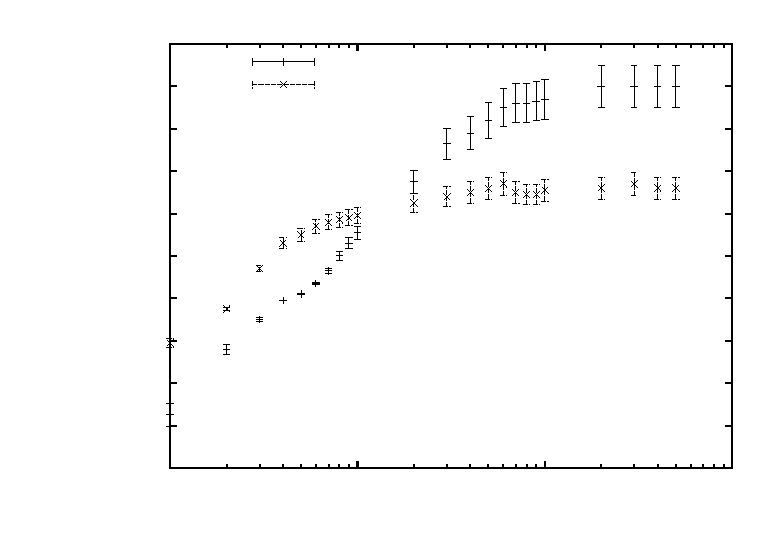
\includegraphics{va}}%
    \gplfronttext
  \end{picture}%
\endgroup

\end{center}
\caption{V-A charakteristika IK}
\label{gVA}
\end{figure}

Na obou křivkách je jasně vidět oblast , která se přibližně chocá dle ohmova zákonu a oblast nasycení. Pto překonání téno oblasti by bylo potřeba vyšší napětí.

\subsection{Svodový proud}
Při napětí 500 V je svodový proud při vzdálenisti elektrod dva centimetry přibližně 50 pA. V případě 6 cm je jeho hodnota ještě o řád nižší, díky čenuž na měření nemá vliv.

\subsection{Střední dolet}
Proměřil jsem podrobněji závislost proudu na vzdálenosti elektrod při napští 
500 V. Hodnoty jsou v tabulce \ref{t2}. Z hodnot je patrné. že při přiblížení 
o více než 4 cm začne proud klesat. To znamená, že se $\alpha$-částicím nepodaří využít celou svou energii k ionizaci. Z toho vyplývá. že jejich dolet je mezi 3 a 4 cm.

\begin{table}
$$
\begin{array}{|c|c|}
d/\mbox{cm}&    I/\mbox{nA} \\ \hline
6&  0.010\\ \hline
5&  0.010\\ \hline
4&  0.010\\ \hline
3&  0.008\\ \hline
2&  0.0052\\ \hline
1&  0.0027\\ \hline
\end{array}
$$
\caption{Závislost proudu na vzdálenosti elektrod při napětí 500 V}
\label{t2}
\end{table}



\subsection{GM}
Zapojit jsem GM dle návodu v \cite{text} a za pomoci osciloskopu proměřil 
jeho V-A charakteristiku. Měřená veličina sice není proud, ale napětí. 
Přepočet je možný za pomoci Ohmova zákona při znalosti odporu osciloskopu, 
který byl 1 M$\Omega$. Nás však zajímá pouze průběh této závislosti, proto přepočet není nutný. Hodnoty jsou v tabulce \ref{tVA2} a na obrázku \ref{gVA2}.
V grafu je jasně zřetelná oblast začátku lavinovité ionizace.
\begin{table}
$$
\begin{array}{|c|c|}
\hline
U_z/\mbox{kV}&    U_s/\mbox{V} \\ \hline
6&  0.0 \\ \hline
7&  0.4 \\ \hline
8&  0.6 \\ \hline
9&  1.0 \\ \hline
10& 2.6 \\ \hline
11& 6 \\ \hline
12& 15 \\ \hline
13& 36 \\ \hline
14& 76 \\ \hline
14.1& 80 \\ \hline
14.2&   80 \\ \hline
14.3&   96 \\ \hline
14.4&   108 \\ \hline
14.5&   130 \\ \hline
14.6&   150 \\ \hline
14.7&   180 \\ \hline
14.8&   210 \\ \hline
14.9&   250 \\ \hline
15.0&   290 \\ \hline
\end{array}
$$
\caption{V-A charakteristika GM}
\label{tVA2}
\end{table}

\begin{figure}
\begin{center}
% GNUPLOT: LaTeX picture with Postscript
\begingroup
  \makeatletter
  \providecommand\color[2][]{%
    \GenericError{(gnuplot) \space\space\space\@spaces}{%
      Package color not loaded in conjunction with
      terminal option `colourtext'%
    }{See the gnuplot documentation for explanation.%
    }{Either use 'blacktext' in gnuplot or load the package
      color.sty in LaTeX.}%
    \renewcommand\color[2][]{}%
  }%
  \providecommand\includegraphics[2][]{%
    \GenericError{(gnuplot) \space\space\space\@spaces}{%
      Package graphicx or graphics not loaded%
    }{See the gnuplot documentation for explanation.%
    }{The gnuplot epslatex terminal needs graphicx.sty or graphics.sty.}%
    \renewcommand\includegraphics[2][]{}%
  }%
  \providecommand\rotatebox[2]{#2}%
  \@ifundefined{ifGPcolor}{%
    \newif\ifGPcolor
    \GPcolorfalse
  }{}%
  \@ifundefined{ifGPblacktext}{%
    \newif\ifGPblacktext
    \GPblacktexttrue
  }{}%
  % define a \g@addto@macro without @ in the name:
  \let\gplgaddtomacro\g@addto@macro
  % define empty templates for all commands taking text:
  \gdef\gplbacktext{}%
  \gdef\gplfronttext{}%
  \makeatother
  \ifGPblacktext
    % no textcolor at all
    \def\colorrgb#1{}%
    \def\colorgray#1{}%
  \else
    % gray or color?
    \ifGPcolor
      \def\colorrgb#1{\color[rgb]{#1}}%
      \def\colorgray#1{\color[gray]{#1}}%
      \expandafter\def\csname LTw\endcsname{\color{white}}%
      \expandafter\def\csname LTb\endcsname{\color{black}}%
      \expandafter\def\csname LTa\endcsname{\color{black}}%
      \expandafter\def\csname LT0\endcsname{\color[rgb]{1,0,0}}%
      \expandafter\def\csname LT1\endcsname{\color[rgb]{0,1,0}}%
      \expandafter\def\csname LT2\endcsname{\color[rgb]{0,0,1}}%
      \expandafter\def\csname LT3\endcsname{\color[rgb]{1,0,1}}%
      \expandafter\def\csname LT4\endcsname{\color[rgb]{0,1,1}}%
      \expandafter\def\csname LT5\endcsname{\color[rgb]{1,1,0}}%
      \expandafter\def\csname LT6\endcsname{\color[rgb]{0,0,0}}%
      \expandafter\def\csname LT7\endcsname{\color[rgb]{1,0.3,0}}%
      \expandafter\def\csname LT8\endcsname{\color[rgb]{0.5,0.5,0.5}}%
    \else
      % gray
      \def\colorrgb#1{\color{black}}%
      \def\colorgray#1{\color[gray]{#1}}%
      \expandafter\def\csname LTw\endcsname{\color{white}}%
      \expandafter\def\csname LTb\endcsname{\color{black}}%
      \expandafter\def\csname LTa\endcsname{\color{black}}%
      \expandafter\def\csname LT0\endcsname{\color{black}}%
      \expandafter\def\csname LT1\endcsname{\color{black}}%
      \expandafter\def\csname LT2\endcsname{\color{black}}%
      \expandafter\def\csname LT3\endcsname{\color{black}}%
      \expandafter\def\csname LT4\endcsname{\color{black}}%
      \expandafter\def\csname LT5\endcsname{\color{black}}%
      \expandafter\def\csname LT6\endcsname{\color{black}}%
      \expandafter\def\csname LT7\endcsname{\color{black}}%
      \expandafter\def\csname LT8\endcsname{\color{black}}%
    \fi
  \fi
  \setlength{\unitlength}{0.0500bp}%
  \begin{picture}(7200.00,5040.00)%
    \gplgaddtomacro\gplbacktext{%
      \csname LTb\endcsname%
      \put(1078,704){\makebox(0,0)[r]{\strut{}-50}}%
      \put(1078,1286){\makebox(0,0)[r]{\strut{} 0}}%
      \put(1078,1867){\makebox(0,0)[r]{\strut{} 50}}%
      \put(1078,2449){\makebox(0,0)[r]{\strut{} 100}}%
      \put(1078,3030){\makebox(0,0)[r]{\strut{} 150}}%
      \put(1078,3612){\makebox(0,0)[r]{\strut{} 200}}%
      \put(1078,4193){\makebox(0,0)[r]{\strut{} 250}}%
      \put(1078,4775){\makebox(0,0)[r]{\strut{} 300}}%
      \put(1210,484){\makebox(0,0){\strut{} 6}}%
      \put(1839,484){\makebox(0,0){\strut{} 7}}%
      \put(2468,484){\makebox(0,0){\strut{} 8}}%
      \put(3096,484){\makebox(0,0){\strut{} 9}}%
      \put(3725,484){\makebox(0,0){\strut{} 10}}%
      \put(4354,484){\makebox(0,0){\strut{} 11}}%
      \put(4983,484){\makebox(0,0){\strut{} 12}}%
      \put(5611,484){\makebox(0,0){\strut{} 13}}%
      \put(6240,484){\makebox(0,0){\strut{} 14}}%
      \put(6869,484){\makebox(0,0){\strut{} 15}}%
      \put(308,2739){\rotatebox{-270}{\makebox(0,0){\strut{}U$_s$/V}}}%
      \put(4039,154){\makebox(0,0){\strut{}U$_z$/kV}}%
    }%
    \gplgaddtomacro\gplfronttext{%
    }%
    \gplbacktext
    \put(0,0){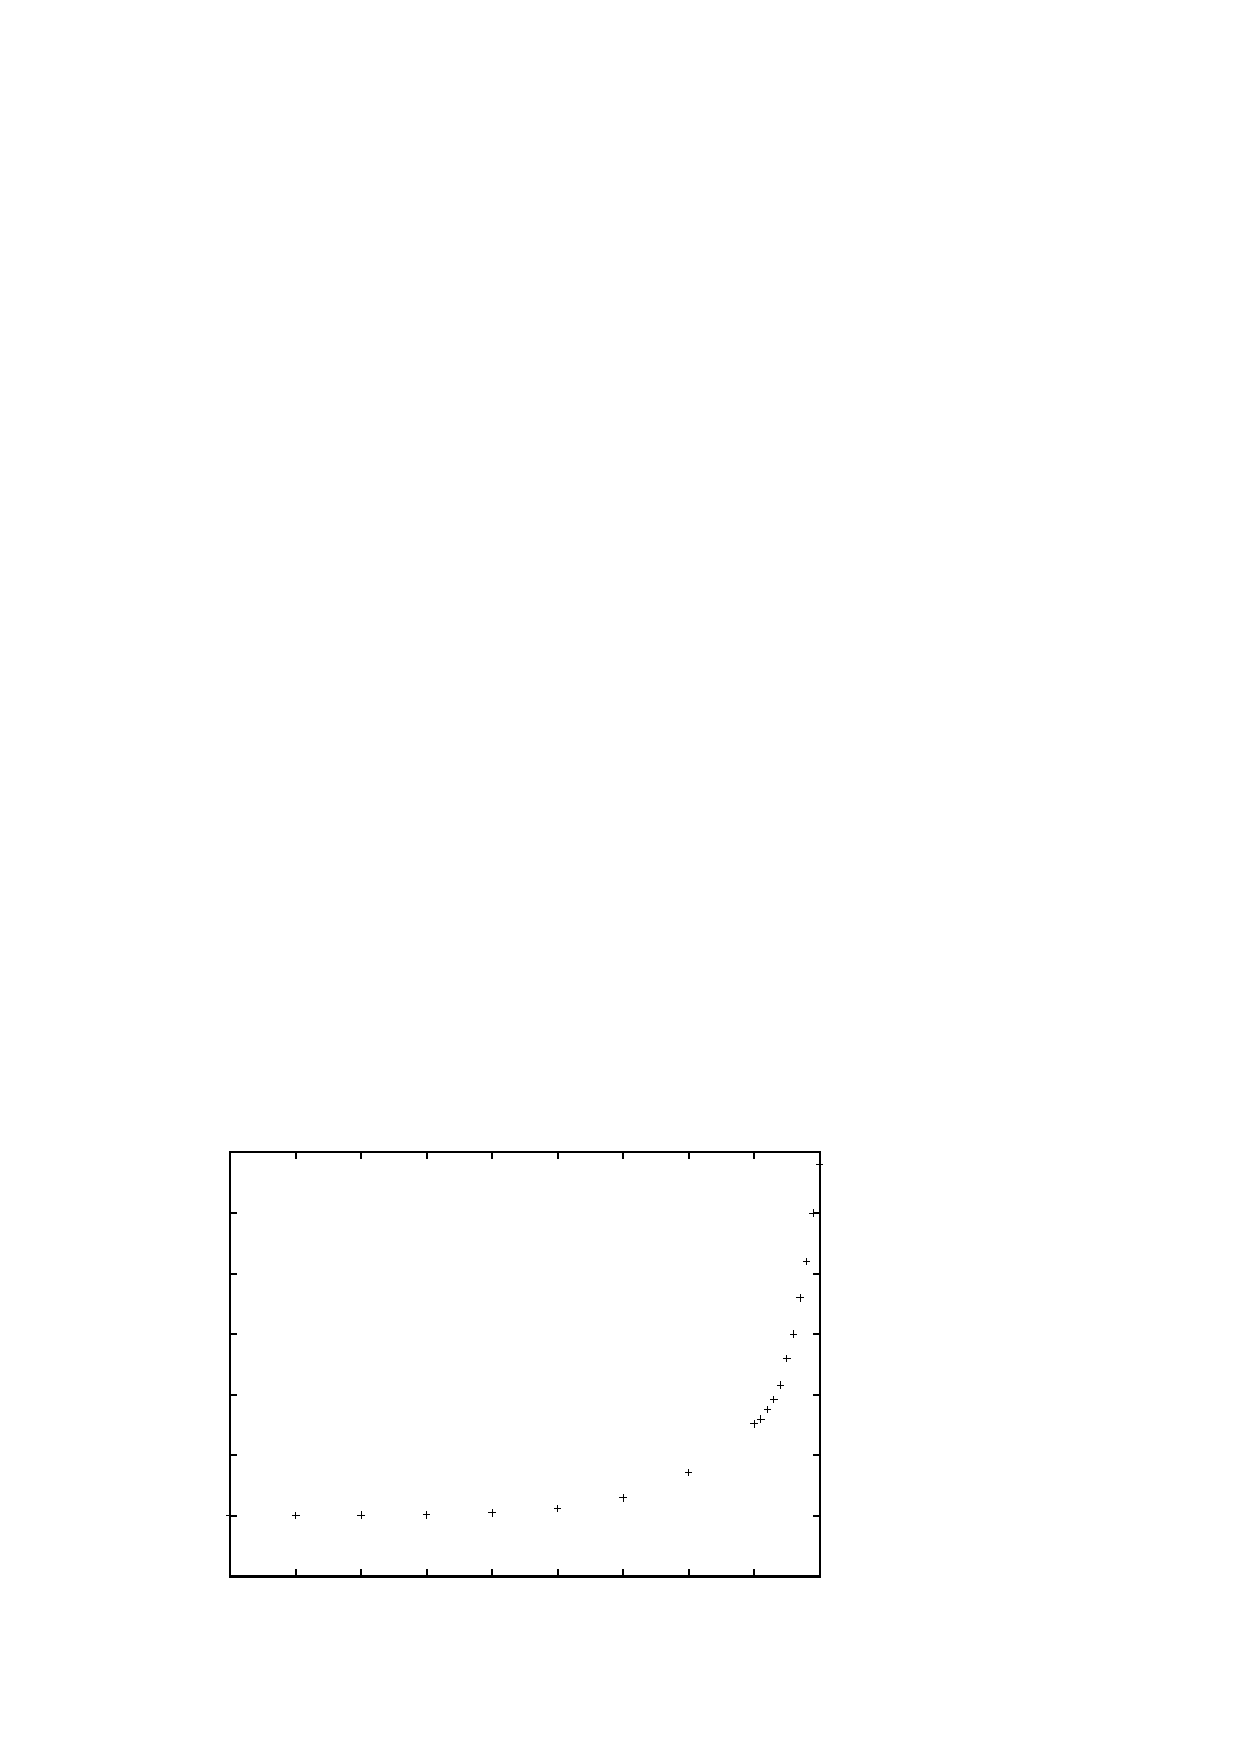
\includegraphics{va2}}%
    \gplfronttext
  \end{picture}%
\endgroup

\end{center}
\caption{V-A charakteristika GM}
\label{gVA2}
\end{figure}


\section{Diskuze}
Určení aktivnějšího vzorku bylo bez problému díky řádovému rozdílu v proudu. Kdyby však byly jejich o něco bližší, vzhledem k fluktuaci proudu by bylo značně obtížné určit rozdíl jejich aktivit.

Při měření V-A charakteristiky IK se ukázalo, že získáme výrazně lepší 
(více se shodující s teoriíú výsledky, pokud postupujeme od nižšího napětí k vyššímu. V opačném případě totiž příležitostně došlo ke skoku v proudu.

Dolet $\alpha$-částic jsme nemohli určit přesněji, protože elektrody umožňovali pohyb pouze o celé centimetry.

U V-A charakteristiky GM jsem hodnoty do 5 kV neuváděl, protože velikost signálu byla neměřitelná osciloskopem.


\section{Závěr}
Určil jsem silnější z přiložených vzorků. \\
Změřil jsem V-A charakteristiku IK. Výsledky jsou v tabulce \ref{tVA} a na obrázku \ref{gVA}. \\
Idetifikoval jsem charakteristivké oblasti v V-A charakteristice IK. \\
Změřil jsem závislost svodového proudu. Výsleky jsou uvedeny výše. \\
Aktivnější vzorek byl zhruba desetkrát aktivnější než slabší. Odhad absolutní aktivity vzorků je
\begin{eqnarray}
A_1=10^6 \mbox{Bq} \\
A_2=10^5 \mbox{Bq}
\end{eqnarray}
Stanovil jsem dolet $\alpha$-částic na 3 až 4 cm. \\
Změřil jsem V-A charakteristiku GM. Výsledky jsou v tabulce \ref{tVA2} na obrázku \ref{gVA2}.

\begin{thebibliography}{5}
	\bibitem{text} \textbf{Studijní text na praktikum IV} \\http://physics.mff.cuni.cz/vyuka/zfp/txt\_402.pdf (23. 10. 2012)
    \bibitem{chyba} \emph{J. Englich}: \textbf{Zpracování výsldků fyzikálních měření} \\ LS 1999/2000
\end{thebibliography}


\end{document}
